%%%%%%%%%%%%%%%%%%%PAPER
%%%%%%%%%%%%%%%%%%%%%%%%%%%%%%%%%%%%%%%%%%%%%%%%%%%%%%%%%%%%%%%%%%%%%%%%%%%%%%%%%%%%%%%%%%%%%%%%%%%%%%%%%%%%%%%%%%%%%%%%%%%%%%%%%%%%%%%%%%%%%
\subsection{Rapidly rotating BEC}
%%%%%%%%%%%%%%%%%%%%%%%%%%%%%%%%%%%%%%%%%%%%%%%%%%%%%%%%%%%%%%%%%%%%%%%%%%%%%%%%%%%%%%%%%%%%%%%%%%%%%%%%%%%%%%%%%%%%%%%%%%%%%%%%%%%%%%%%%%%%%
For this work, we numerically solve the Gross-Pitaevskii equation in two dimensions, assuming a strong confinement along the third axis.
This allows all dynamics to be restricted to the $xy$ plane, with vortices behaving as charged particles in a neutral background. In the
frame corotating with the condensate, this can be modeled as
\begin{equation}
	 i\hbar\partial_t \Psi\left(\mathbf{x},t\right) = \left[ -\frac{\hbar^2}{2m}\nabla^2 + V\left(\mathbf{x}\right) + g\vert \Psi\left(\mathbf{x},t\right) \vert^2 - \Omega L_z \right]\Psi\left(\mathbf{x},t\right)
\end{equation}
where $V\left(\mathbf{x}\right)$ is the trapping geometry, $\Omega$ is the trap rotation frequency, and $L_z$ is the angular momentum
operator along the $z$-direction. For the rapidly rotating case, the vortices form an ordered triangular lattice, that rotates equivalently
to a solid-body in the large number limit. Deviations from the solid-body rotation can be seen for trajectories in the limit of long times
(~10 s). This is very likely due to long-wavelength Tkachenko modes in the condensate, and following the analysis of [Baym, Tk modes of vtx latt in rr BEC]
has a frequency much longer than the lifetime of the system for our given rotation rate.
%However, due to the density inhomogeneities of a harmonically trapped condensate, and the likelihood of shearing this is (I think) expected.
The lattice is well ordered and behaved at timescales on the order of upto few seconds, as well as away from the condensate edges, and so we
will restrict our analysis therein.

As condensates are highly controllable in the lab (cite many papers), we consider the use of many common experimental techniques to engineer
specific states otherwise difficult in solid-state materials. One such set of systems are those of crystals with controllable defects, which
although (relatively) easily created classically (cite bead packing, etc), are difficult experimentally in quantum systems due to the sizes
of interatomic spacings. Here we propose the use of phase-imprinting (cite) as a means of achieving such defects in a Bose-Einstein
condensate. Through direct manipulation of the condensate phase, vortices may be added or removed from specific locations in the system.

%%%%%%%%%%%%%%%%%%%%%%%%%%%%%%%%%%%%%%%%%%%%%%%%%%%%%%%%%%%%%%%%%%%%%%%%%%%%%%%%%%%%%%%%%%%%%%%%%%%%%%%%%%%%%%%%%%%%%%%%%%%%%%%%%%%%%%%%%%%%%
\subsection{Order/disorder}
%%%%%%%%%%%%%%%%%%%%%%%%%%%%%%%%%%%%%%%%%%%%%%%%%%%%%%%%%%%%%%%%%%%%%%%%%%%%%%%%%%%%%%%%%%%%%%%%%%%%%%%%%%%%%%%%%%%%%%%%%%%%%%%%%%%%%%%%%%%%%
Given the localised defect disturbs the lattice after sufficiently long times, we can examine if the lattice moves from global ordered to
disordered following the addition or removal of another site over the course of time. For a two-dimensional material, KTHNY theory describes
the transitions from a solid crystalline to amorphous fluid phase, via an intermediate hexatic phase. This state is generally characterised
by the translational and orientational correlation functions long-ranged behaviour. As we have an inhomogeneous density profile, and thus
lattice outside a given radius, the use of translational correlations does not make much sense. Orientational correlations however, which
measure how the lattice aligns to a particular angle, should suffice when combined with the density structure factor,
$S = \int d\mathbf{r}e^{i\mathbf{k}\cdot\mathbf{r}}|\Psi|^2$. True crystalline behaviour is given by orientational constant values, with
power-law decay is expected for a hexatic phase, and exponential decay for an amorphous fluid (neglecting translational correlations).

%%%%%%%%%%%%%%%%%%%%%%%%%%%%%%%%%%%%%%%%%%%%%%%%%%%%%%%%%%%%%%%%%%%%%%%%%%%%%%%%%%%%%%%%%%%%%%%%%%%%%%%%%%%%%%%%%%%%%%%%%%%%%%%%%%%%%%%%%%%%%
\subsection{Phase imprinting defects}
%%%%%%%%%%%%%%%%%%%%%%%%%%%%%%%%%%%%%%%%%%%%%%%%%%%%%%%%%%%%%%%%%%%%%%%%%%%%%%%%%%%%%%%%%%%%%%%%%%%%%%%%%%%%%%%%%%%%%%%%%%%%%%%%%%%%%%%%%%%%%
Phase imprinting has been shown as an effective tool for the creation of vortices within a Bose-Einstein condensate (cite). The signature of
a quantum vortex is given by a phase singularity, around which the phase winds through $\pm 2\pi$, depending upon the direct of rotation.
Through the use of the phase imprinting method, we can eliminate a vortex from the lattice by applying the correct phase profile. To
eliminate a vortex from the lattice we need only to apply the opposite phase winding to that of the vortex to be eliminated. The
instantaneous application of a phase singularity to the condensate will create phonon modes in the density, as will the annihilation event.
Since the induced phonons have been shown to yield minimal impact on the vortex lattice structure <ref my paper>, we can safely
ignore their contribution. The removal of a vortex from the lattice introduces a vacancy to the system.


We model the vortex lattice as a graph, where each vortex represents a node, and edges are given by nearest neighbours at most separated by
a distance $a_v$, for a triangular lattice configuration, or $\sqrt{2}a_v$ for a square lattice (see Fig. \ref{fig:vtxdist}). The inclusion
of the square lattice distance is chosen so that upon removal, the vortices can reconfigure their arrangement locally, and may move from
triangular to square geometries. As they behave like Coulombic particles with a profile that falls off as $r^{-1}$ we can consider that any
interactions outside these distances to be negligible.

\subsubsection{Lattice vacancy}
%%%%%%%%%%%%%%%%%%%%%%%%%%%%%%%%%%%%%%%%%%%%%%%%%%%%%%%%%%%%%%%%%%%%%%%%%%%%%%%%%%%%%%%%%%%%%%%%%%%%%%%%%%%%%%%%%%%%%%%%%%%%%%%%%%%%%%%%%%%%%
The removal of a vortex from the vortex is thus expected to affect only the nearest neighbours by altering their velocity well, with the
overall angular momentum of the condensate decremented by a single quantum. The resulting vacancy, following a vortex removal, remains
localised to its respective position within the lattice for long times, regardless of initial placement (assuming not at edge)
(see Fig. \ref{fig:trajectory}). The
resulting stability of the nearest neighbours follows a decay of the honeycomb-like structure akin to that described by [statistical
topology of perturbed two-dimensional lattices]. Given enough time, this structure decays via one of the three possible means, creating a
locally disordered region with a grain boundary/disclination/dislocation? evident of the lattice change. However, even for long times, the
overall vortex lattice remains well structured, as evidenced by examining correlation functions of the vortex positions for both two-body,
and orientational correlations.


\iffalse
\include{g6rimg}
\fi

After the vortex removal, the system remains in a stable configuration, for a period on the order of 100+ ms (see Fig. \ref{fig:voronoi_area},
\ref{fig:voronoi_100ms}), after which the vortices begin to deviate from their lattice positions and attempt to fill the vacancy and balance
the inter-vortex forces.
\iffalse
\begin{figure}[tb]
	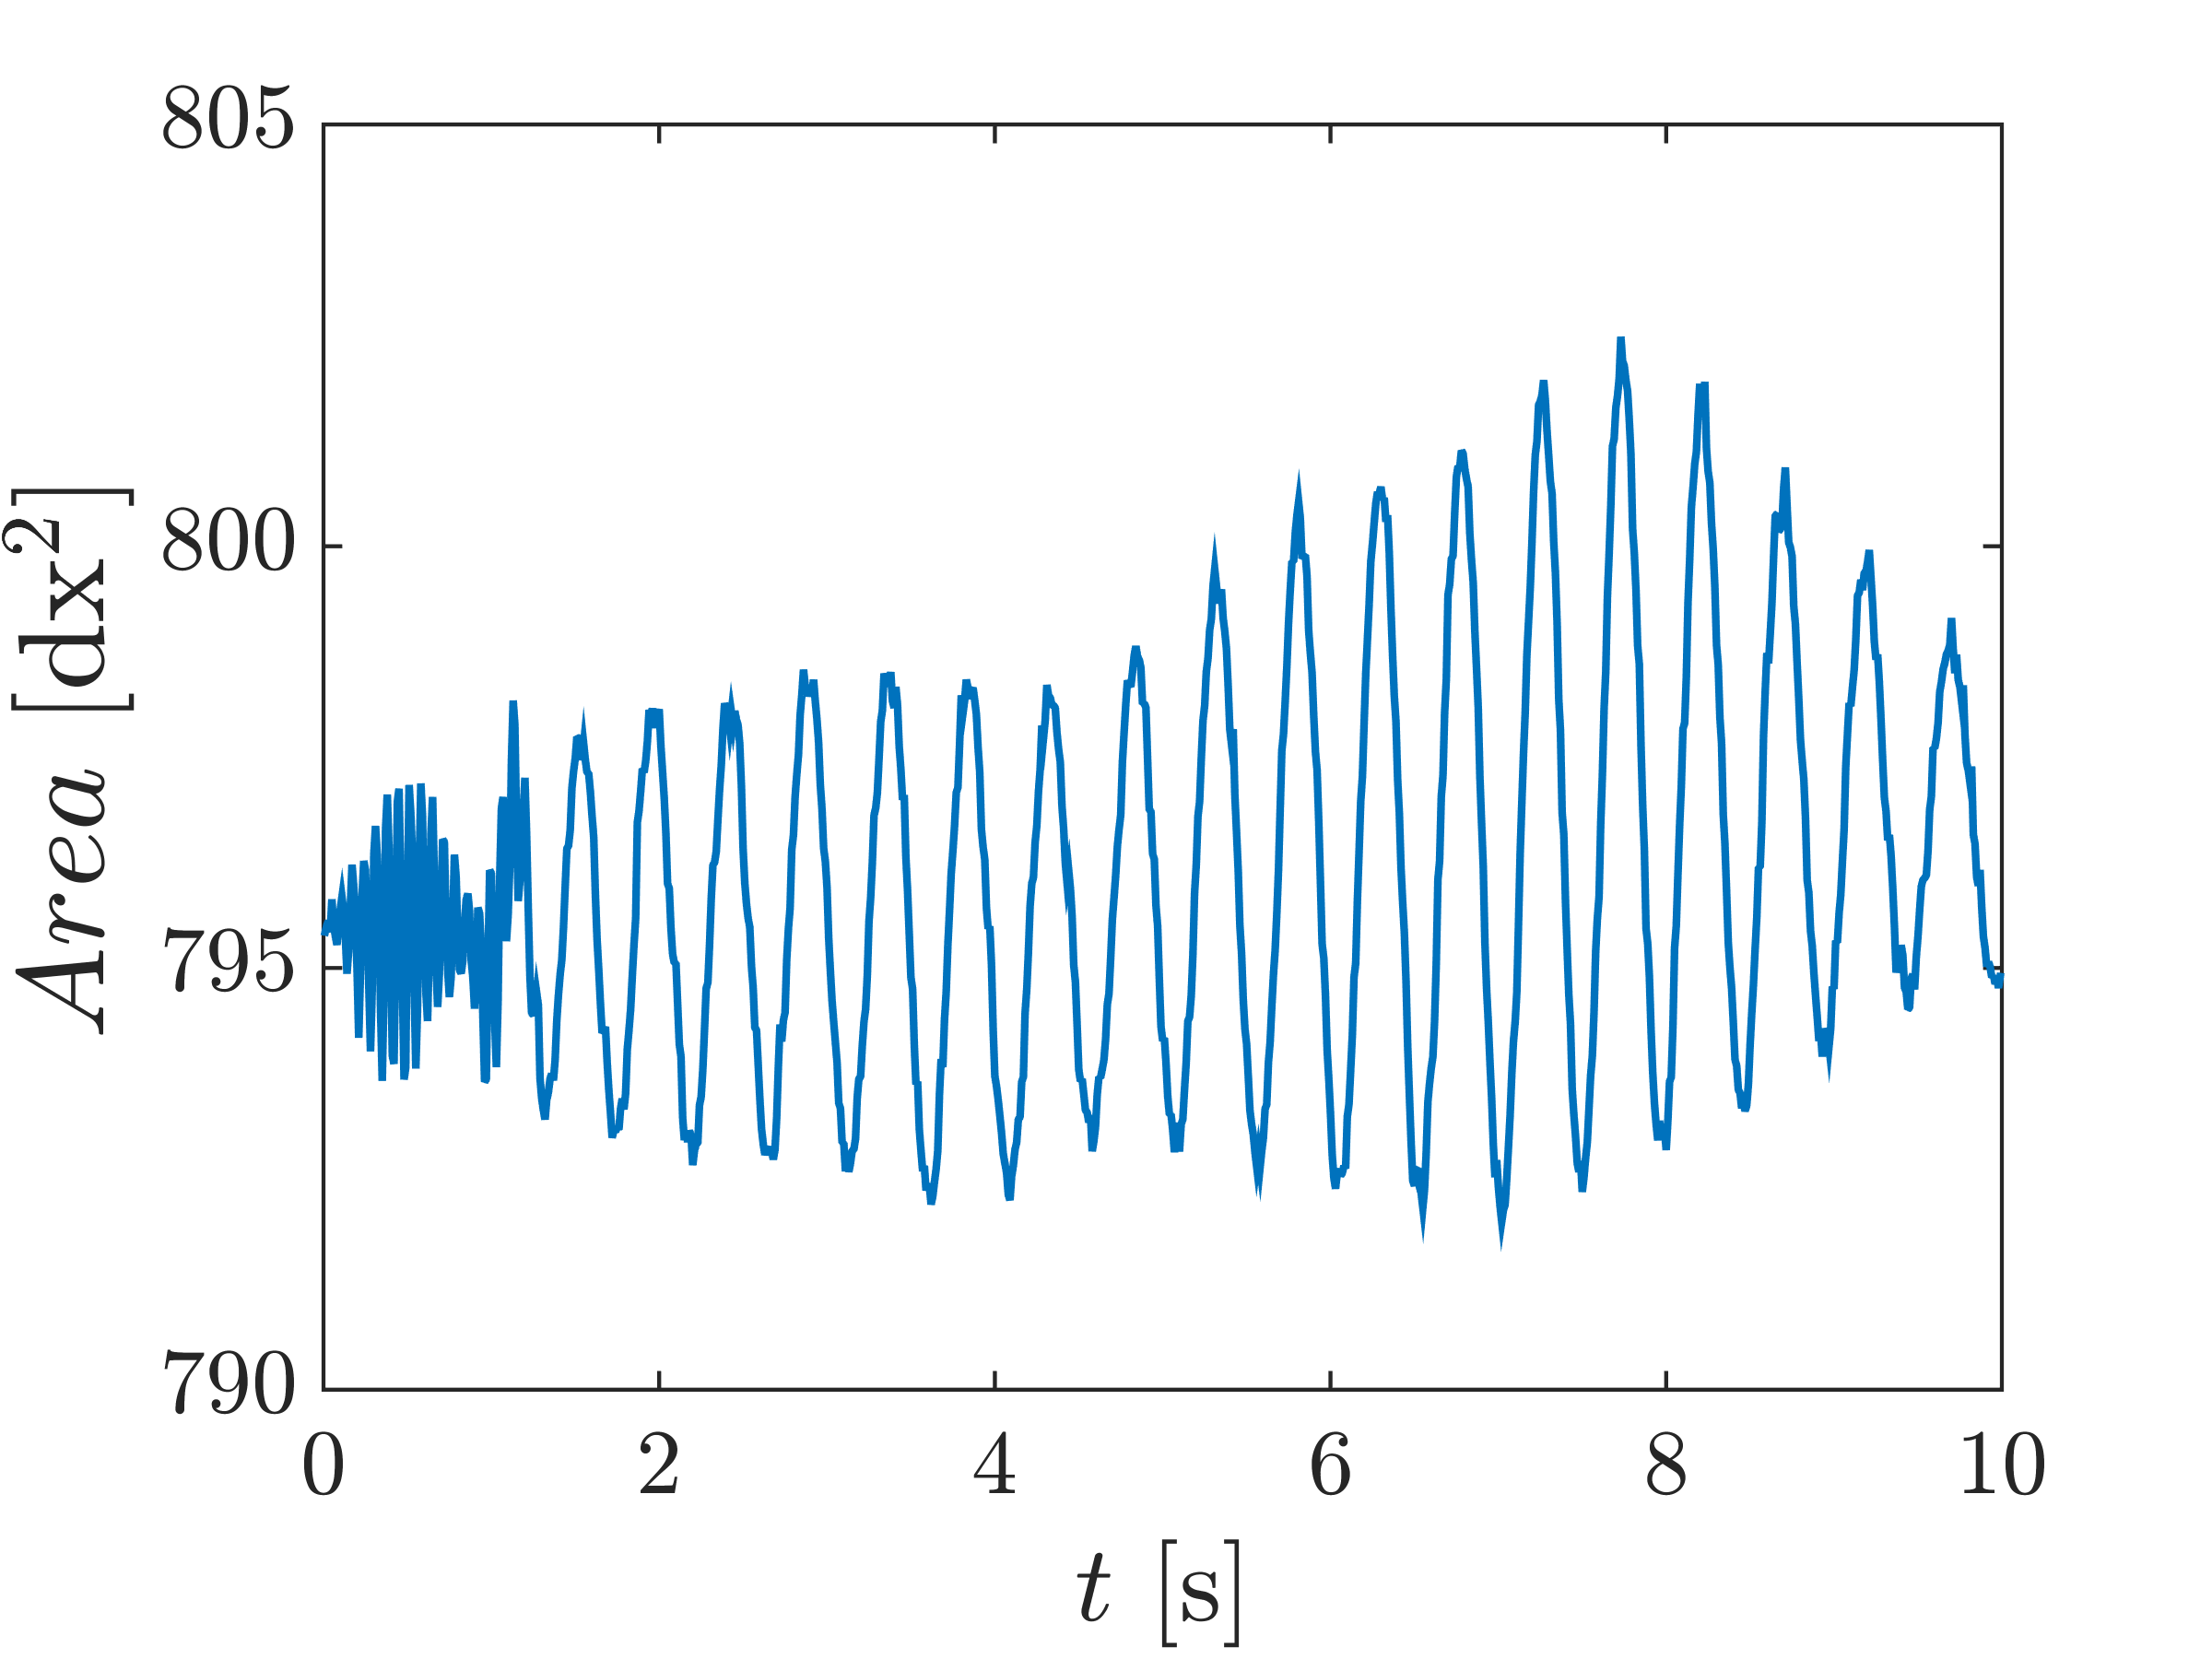
\includegraphics[width=0.48\textwidth]{imgs/Disloc_-1_centre_avgarea}
	\caption{Voronoi cell average area after removing vortex at condensate centre. }
	\label{fig:voronoi_area}
\end{figure}
\fi
Removing vortices at different positions in the lattice shows similar behaviour, with the effect on the velocity profile and trajectories of
other vortices being mostly localised around the removal site.

\iffalse
\begin{figure}[tb]
	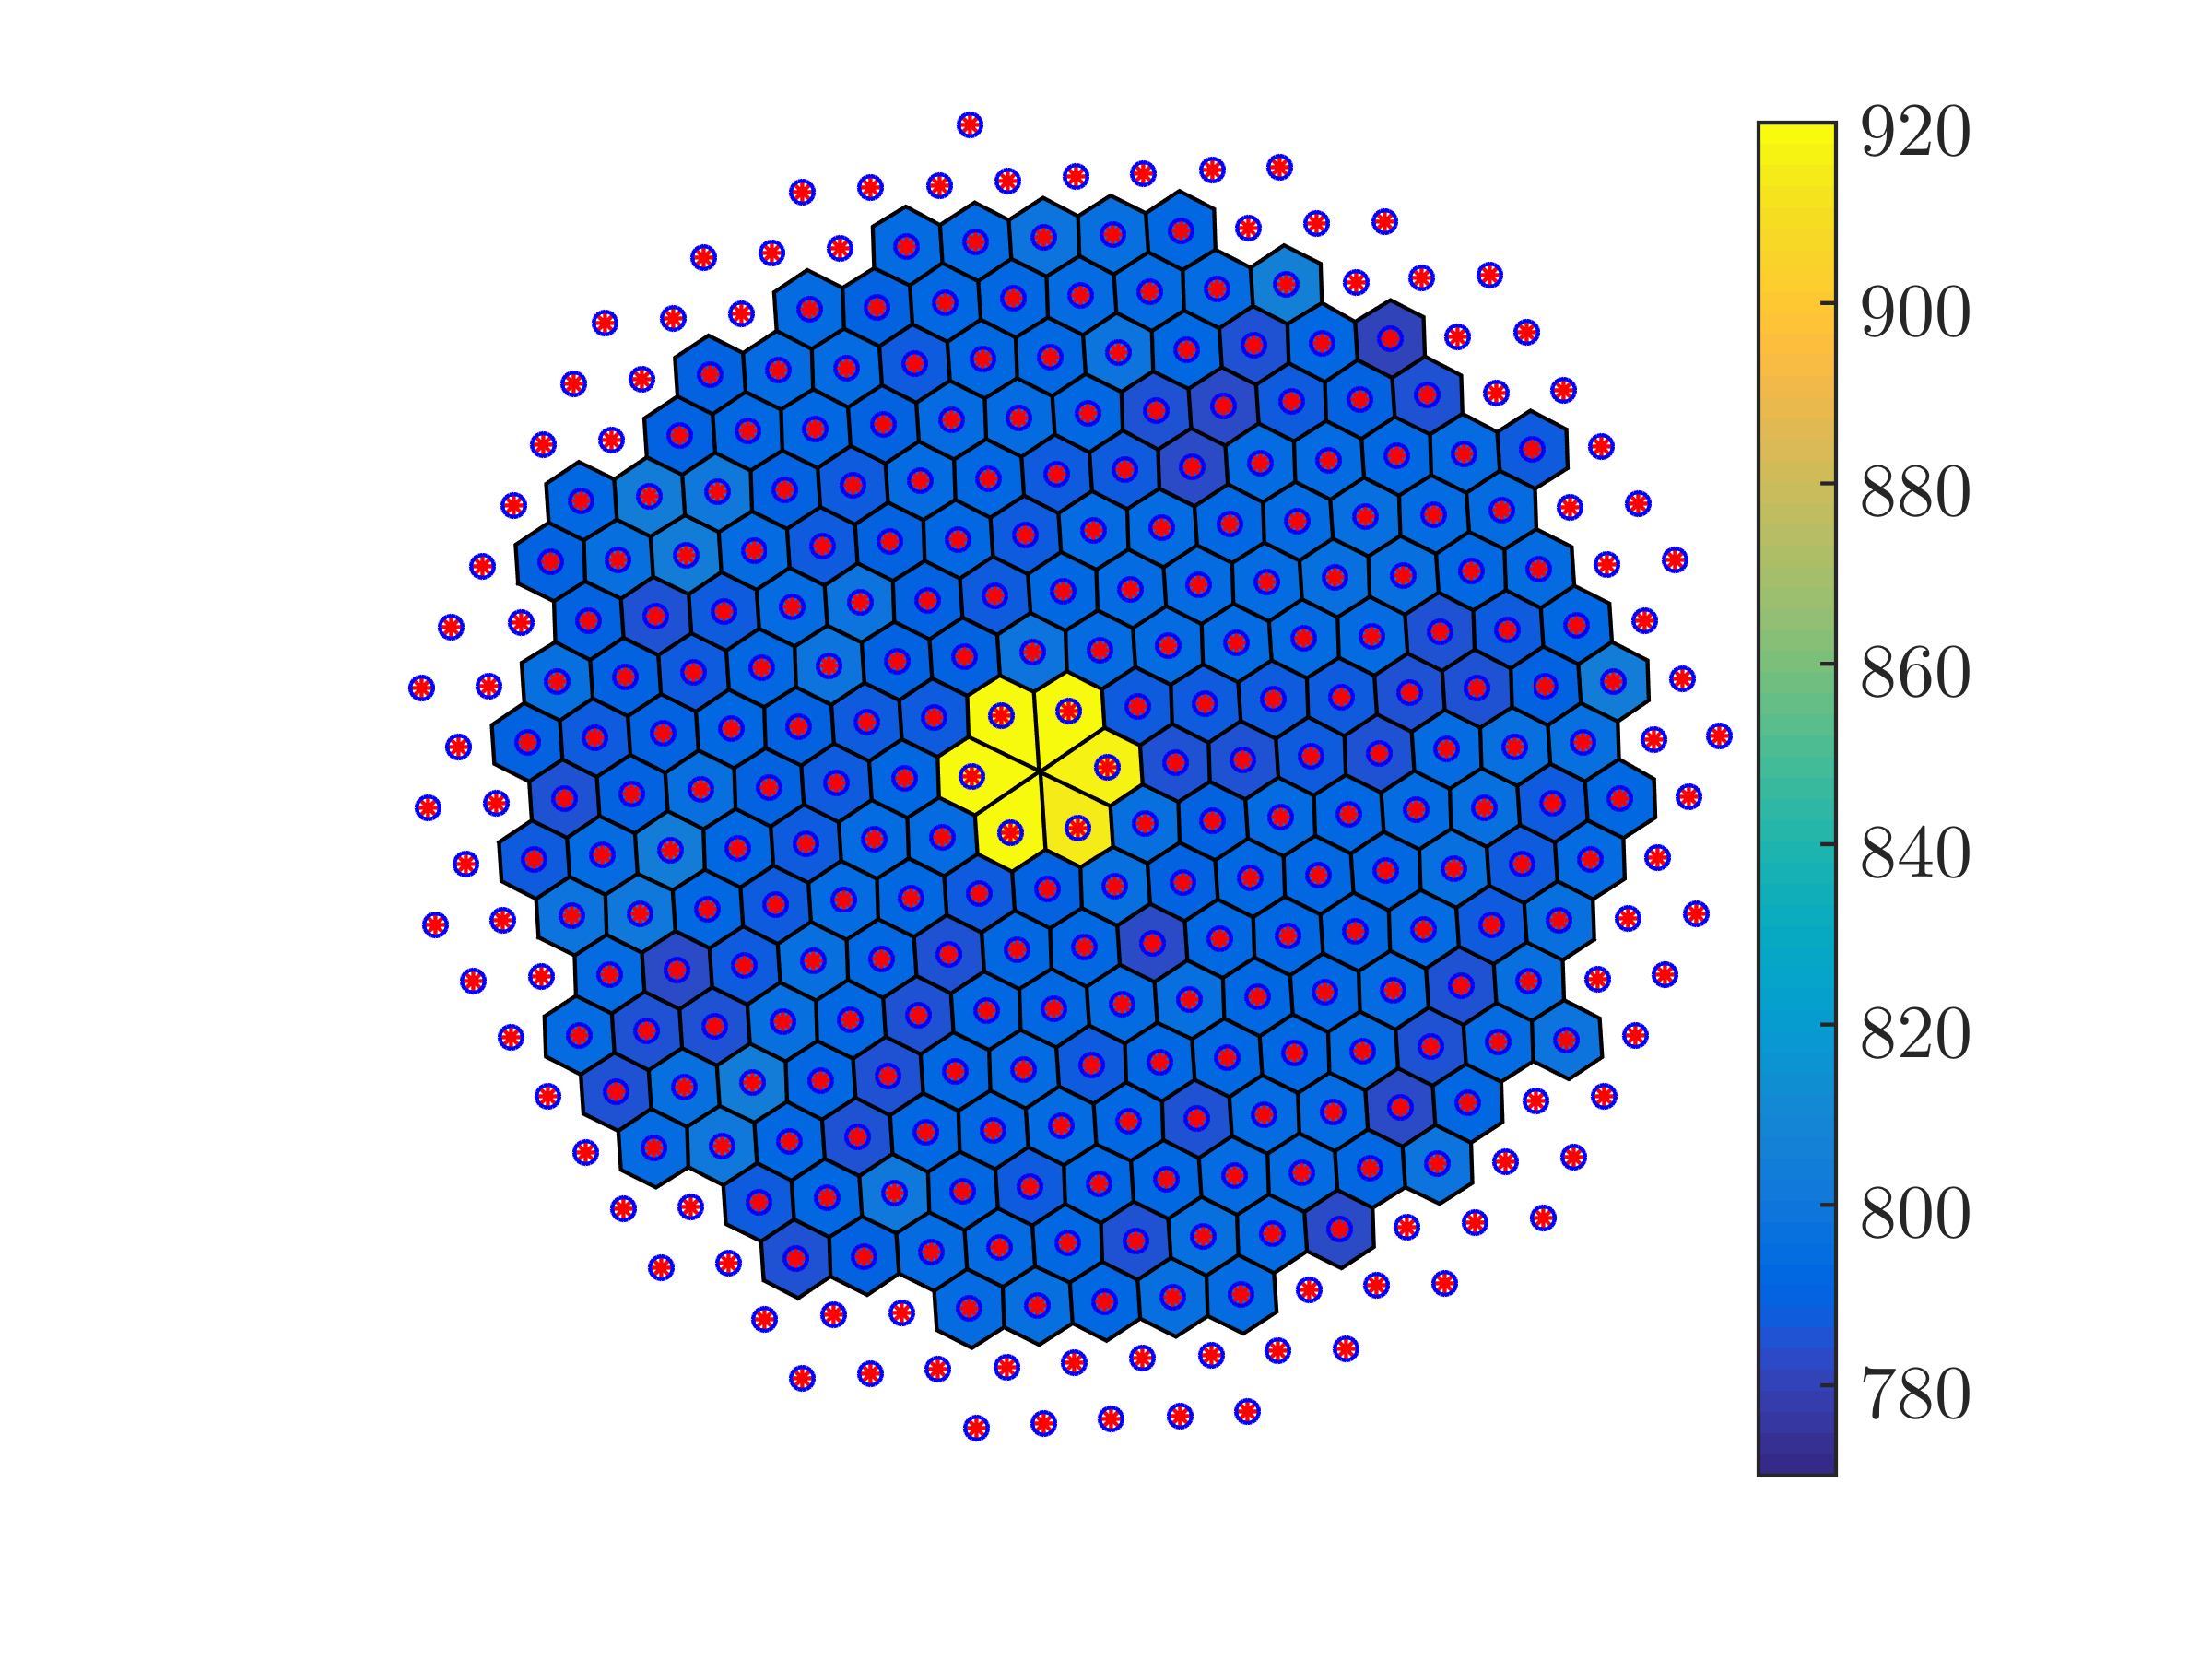
\includegraphics[width=0.48\textwidth]{imgs/Disloc_-1_centre_voronoi_t100ms_cbar}
	\caption{Voronoi cells after removing vortex at condensate centre for t=100 ms. Vortices at edge boundary neglected. }
	\label{fig:voronoi_100ms}
\end{figure}
\fi
Tracking the vortex distances traveled for different removal locations, and for a different number of removed vortices shows how much we
disturb the underlying lattice (see \ref{fig:vtxdist}).

\iffalse
\begin{figure}[tb]
	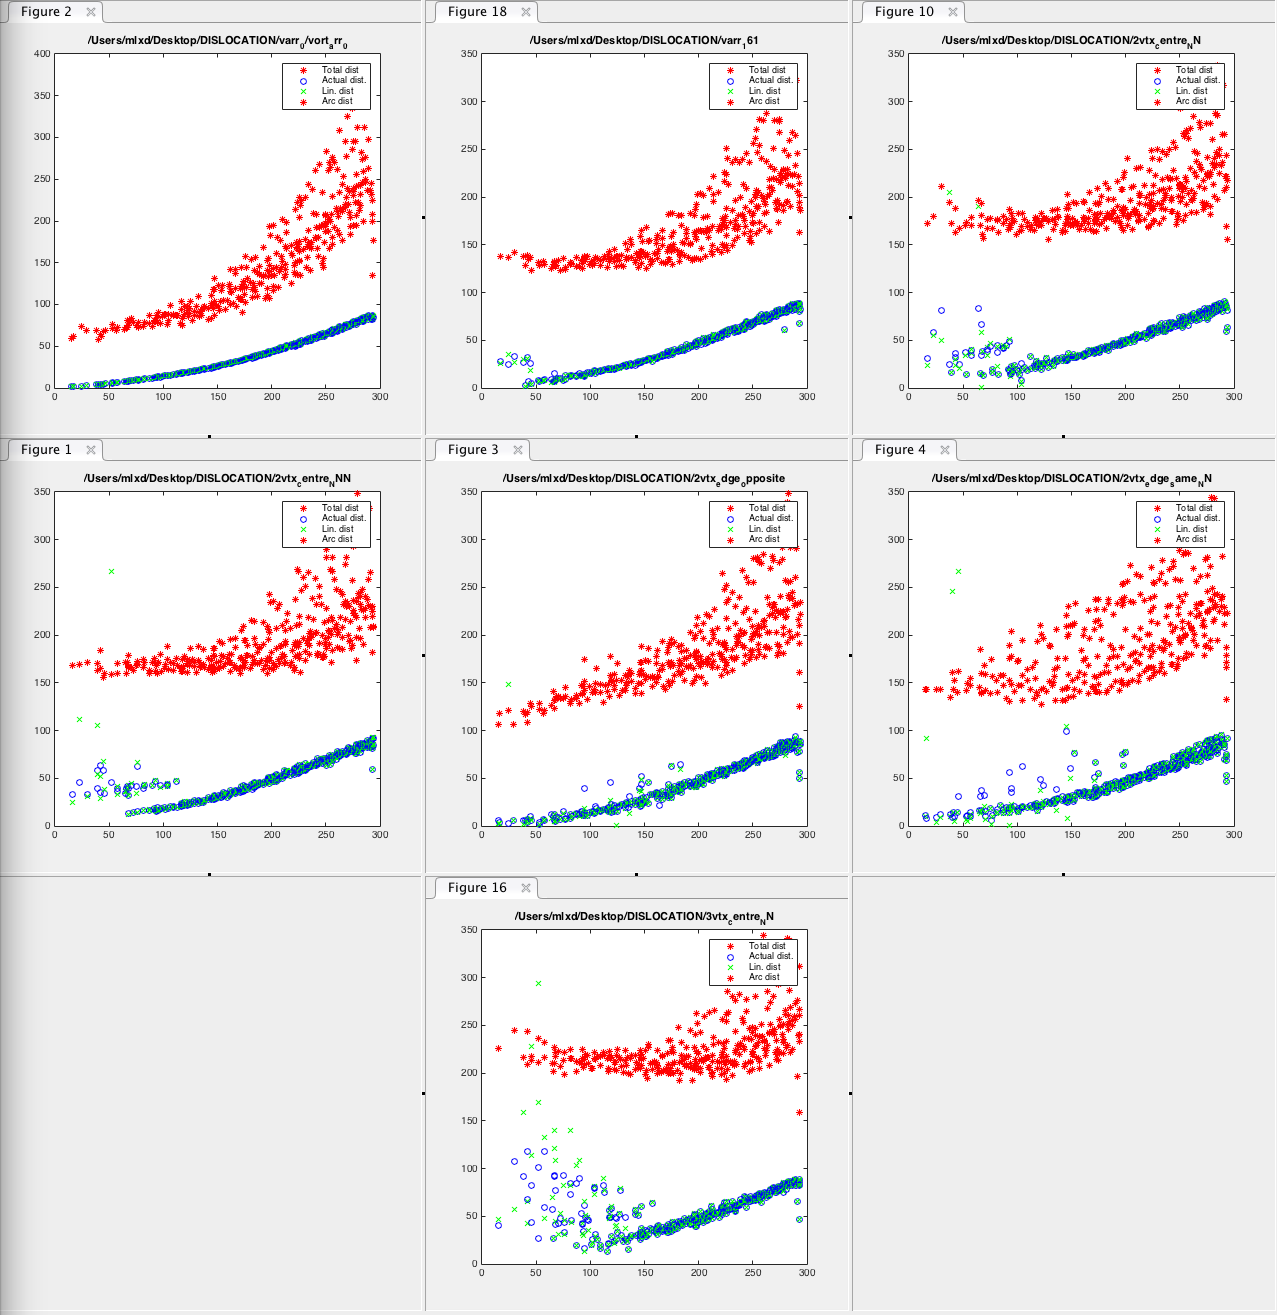
\includegraphics[width=0.48\textwidth]{imgs/vtx_distance_travelled}
	\caption{Vortex total traveled distance with different removal positions for between 1 and 3 vortices.}
	\label{fig:vtxdist}
\end{figure}
\fi



\subsubsection{Lattice overpopulation}
%%%%%%%%%%%%%%%%%%%%%%%%%%%%%%%%%%%%%%%%%%%%%%%%%%%%%%%%%%%%%%%%%%%%%%%%%%%%%%%%%%%%%%%%%%%%%%%%%%%%%%%%%%%%%%%%%%%%%%%%%%%%%%%%%%%%%%%%%%%%%
Similarly to removing a vortex from the lattice, we can also add one. By choosing a pre-existing vortex and adding a like-signed phase
winding, we can create multiply charged vortices in the condensate, where the vortex has a winding of $2\pi l$, with $l$ as the vortex
charge. Multiply charged vortices are usually unstable in condensates, as it is more energetically favourable to have two singly charged
vortices, than a single doubly charged vortex, as the energy increases with $l^2$. Thus, an $l$-charged vortex is expected to instead decay
into $l$ singly-charged vortices due to the presence of complex eigenmodes in the Bogoliubov spectrum \cite{VTX:Kawaguchi_pra_2004}.

Here we have taken our lattice of $l=1$ vortices, and given an additional charge to a single vortex to examine the decay process. However,
the presence of the lattice suppresses the decay process for long times (order of seconds) compared to that of in a condensate without vortex
lattice. The doubly charged vortex remains stable on the order of seconds even away from the lattice centre (though does decay eventually).
The additional velocity profile locally causes the nearest neighbouring vortices to rotate faster than the solid-body rotation rate of the
whole lattice, causing a local shearing of the lattice structure. As with the vacancies, the use of correlation functions allowed us to
examine the short and long-range order of the lattice.

Voronoi diagrams of the resulting lattice show a stable doubly charged vortex position, with show twisting of the lattice about this central
point.

\begin{figure}[tb]
	\includegraphics[width=0.49\textwidth]{imgs/DoubleCharge/add161/voronoi}
	\includegraphics[width=0.49\textwidth]{imgs/DoubleCharge/add161remove207/voronoi}
	\caption{(top) Doubly charged central vortex. Doubly charged vortex remains stable, and retains 6-fold
	symmetry of vortex lattice. (bottom) Doubly charged central vortex, and removal of nearby vortex. Doubly charged vortex remains stable, and forms 8-fold
	symmetry of vortex neighbours.}
	\label{fig:voronoi_double}
\end{figure}



%%%%%%%%%%%%%%%%%%%%%%%%%%%%%%%%%%%%%%%%%%%%%%%%%%%%%%%%%%%%%%%%%%%%%%%%%%%%%%%%%%%%%%%%%%%%%%%%%%%%%%%%%%%%%%%%%%%%%%%%%%%%%%%%%%%%%%%%%%%%%
\subsection{Things to note}
%%%%%%%%%%%%%%%%%%%%%%%%%%%%%%%%%%%%%%%%%%%%%%%%%%%%%%%%%%%%%%%%%%%%%%%%%%%%%%%%%%%%%%%%%%%%%%%%%%%%%%%%%%%%%%%%%%%%%%%%%%%%%%%%%%%%%%%%%%%%%

\begin{itemize}
\item Localised disturbances: introducing vacancy to lattice causes it to travel with lattice. Change in velocity profile only affects 6
nearest neighbours on moderate timescales.
\item Long range hexatic phase has short range translational order (exp drop off), but constant orientational order -> is this such a phase?
\end{itemize}

%%%%%%%%%%%%%%%%%%%%%%%%%%%%%%%%%%%%%%%%%%%%%%%%%%%%%%%%%%%%%%%%%%%%%%%%%%%%%%%%%%%%%%%%%%%%%%%%%%%%%%%%%%%%%%%%%%%%%%%%%%%%%%%%%%%%%%%%%%%%%
\subsection{Correlations}
%%%%%%%%%%%%%%%%%%%%%%%%%%%%%%%%%%%%%%%%%%%%%%%%%%%%%%%%%%%%%%%%%%%%%%%%%%%%%%%%%%%%%%%%%%%%%%%%%%%%%%%%%%%%%%%%%%%%%%%%%%%%%%%%%%%%%%%%%%%%%
According to KTHNY theory for a 2D material the transition from a solid crystal to liquid phase is mediated through an intermediary hexatic
phase. This phase is usually characterised by the translational and orientational correlation functions. Given the lack of translation order
in a harmonically trapped condensate, we restrict our analysis to the orientational correlation function, $g_6$ given by
\iffalse
\begin{equation}
	\begin{aligned}
		g_6(|\mathbf{r}_i - \mathbf{r}_j|) &= \\ \frac{1}{N(r)}\displaystyle\sum_{i}^{N(r)}\displaystyle\sum_{j}^{N(r)} & \left(\frac{1}{n_j}\displaystyle\sum_{k}^{n_j}\exp(6\mathrm{i}\theta_{jk}) \right)\left(\frac{1}{n_i}\displaystyle\sum_{l}^{n_i}\exp(6\mathrm{i}\theta_{il}) \right)^{*}
	\end{aligned}
\end{equation}
\fi
\begin{equation}
	g_6(r) = \frac{1}{N(r)}\displaystyle\sum\limits_{i,j}^{N(r)}\psi_6(\mathbf{r}_i)\psi_6^{*}(\mathbf{r}_j),
\end{equation}
with
\begin{equation}
	\psi_6(|\mathbf{r}_{i} - \mathbf{r}_{j}|) = \frac{1}{n_i}\displaystyle\sum\limits_j^{n_i}\exp(6\mathrm{i}(\theta_i - \theta_j)),
\end{equation}
where $\psi_6$ is the orientational order parameter, and $j$ is over the nearest neighbouring vortices.

According to [] the decay in correlations for both translational and orientational order give indication to the material phase. In a
two-dimensional material the positional order is expected to decay algebraically as a function of radius, differing from that of a
three-dimensional material, which tends to a constant value. Here we examine the orientational correlation function as a measure of the
order of a "vortex unit cell", consisting of the angle made by nearest neighbours to an individual vortex. For a perfectly ordered
triangular lattice this value will tend to 1. To maintain constant vortex areal density, we choose vortices defined at a radius of
$r=2\times 10^4$ m from the centre, which give an almost uniform lattice constant for our system parameters.

\begin{itemize}
\item Crystalline: $\lim\limits_{r\rightarrow \infty}\hat{g}_T(r) \neq 0$, $\lim\limits_{r\rightarrow \infty}\hat{g}_6(r) \neq 0$
\item Long-range hexatic: $\hat{g}_T(r) \approx _{r\rightarrow \infty} \exp(-r/\xi_T) $, $\lim\limits_{r\rightarrow \infty}\hat{g}_6(r) \neq 0$
\item Power-law hexatic: $\hat{g}_T(r) \approx _{r\rightarrow \infty} \exp(-r/\xi_T) $, $\hat{g}_6(r) \approx _{r\rightarrow \infty} 1/r^{\eta_6}$
\item Amorphous: $\hat{g}_T(r) \approx _{r\rightarrow \infty} \exp(-r/\xi_T) $, $\hat{g}_6(r) \approx _{r\rightarrow \infty} \exp(-r/\xi_6) $
\end{itemize}
Hat means normalised (see page 119 of order in two dim binary random arrays, Nelson et al.)


%%%%%%%%%%%%%%%%%%%%%%%%%%%%%%%%%%%%%%%%%%%%%%%%%%%%%%%%%%%%%%%%%%%%%%%%%%%%%%%%%%%%%%%%%%%%%%%%%%%%%%%%%%%%%%%%%%%%%%%%%%%%%%%%%%%%%%%%%%%%%
\subsection{Numerics and results}\label{sec:numerics}
%%%%%%%%%%%%%%%%%%%%%%%%%%%%%%%%%%%%%%%%%%%%%%%%%%%%%%%%%%%%%%%%%%%%%%%%%%%%%%%%%%%%%%%%%%%%%%%%%%%%%%%%%%%%%%%%%%%%%%%%%%%%%%%%%%%%%%%%%%%%%

Each vortex position was found by summing over adjacent grid sites, and looking for a $2\pi$ phase winding. This gave a vortex position
estimated to the numerical grid. A least-squares fit was performed to more accurately determine the vortex core. Vortices closest the centre
of the condensate were considered to ensure an almost uniform inter-vortex spacing, giving minimal deviation in lattice constant, $a_v$. Each
vortex was assigned a unique identifier (UID) to allow for it to be tracked individually over the course of the simulations, with the initial
configuration presented in the graph [ref graph]. By noting these UIDs, vortices can be individually selected for removal by applying the
global $2\pi$ phase winding in the opposing direction, centered on the core.

The trajectory plots show very small global effect on the core positions, with a disturbance localised in a region centered on the removed
core. By removing vortices in different locations on the condensate we see similar behaviour, with the trajectories modified in a region
around the removed vortex. The removal of two vortex adjacent cores can be seen to crate a greater disturbance, as expected, with the
trajectories of the surrounding vortices no longer following an almost circular path (more like hexagonal), but taking on other geometric
path shapes. For two nn vortices the path becomes an almost rhombic shape, with nnn forming an elongated hexagon (as to be expected). For 3
nn, the resulting trajectories follow a triangular pattern of the same orientation as the removed vortices. For the removal of an entire 7
vortex cell, the formed pattern is star shaped.

TODO:
Calculate incompressible kinetic energy spectrum for each case, and see if useful. RESULT: It wasn't.
Calculate $S(k) = |\Psi(k)|^2$ for condensate densities, not just vortex positions, for comparison. RESULT: looks strange, even in untouched
case. Arcs exist in all cases, but with interference lines.

The impact on the overall distances traveled by each vortex as a result of the dislocations is given in figure [some fig].

%\iffalse
\begin{figure}[tb]
	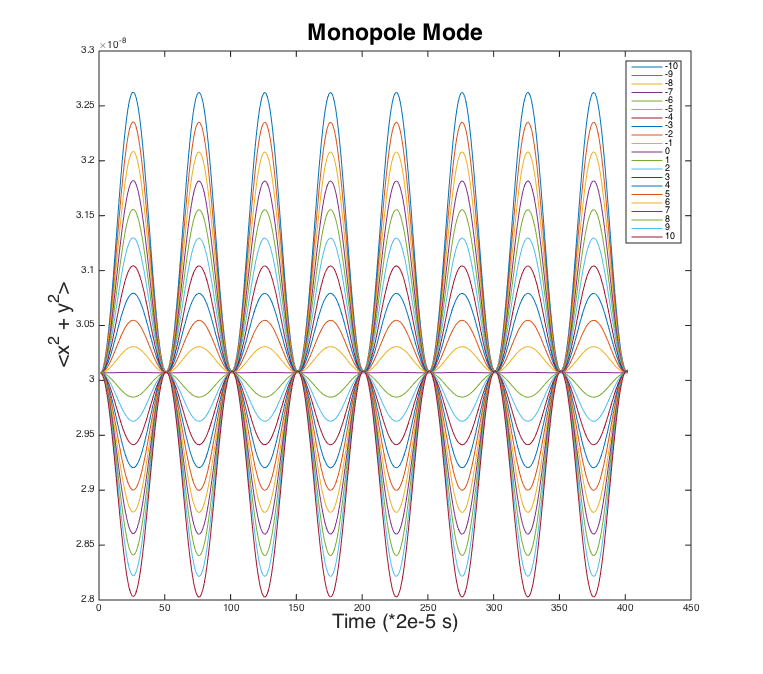
\includegraphics[width=0.48\textwidth]{imgs/mono}
	\caption{The oscillation of the mean-radius of the condensate after the addition of vortices (positive) or antivortices (negative) with
	different imprinted windings. The oscillation mode shows an exact match for a 2D non-rotating condensate of $2\omega_{\perp}$ for all cases.}
\end{figure}
%\fi

\begin{figure}[tb]
	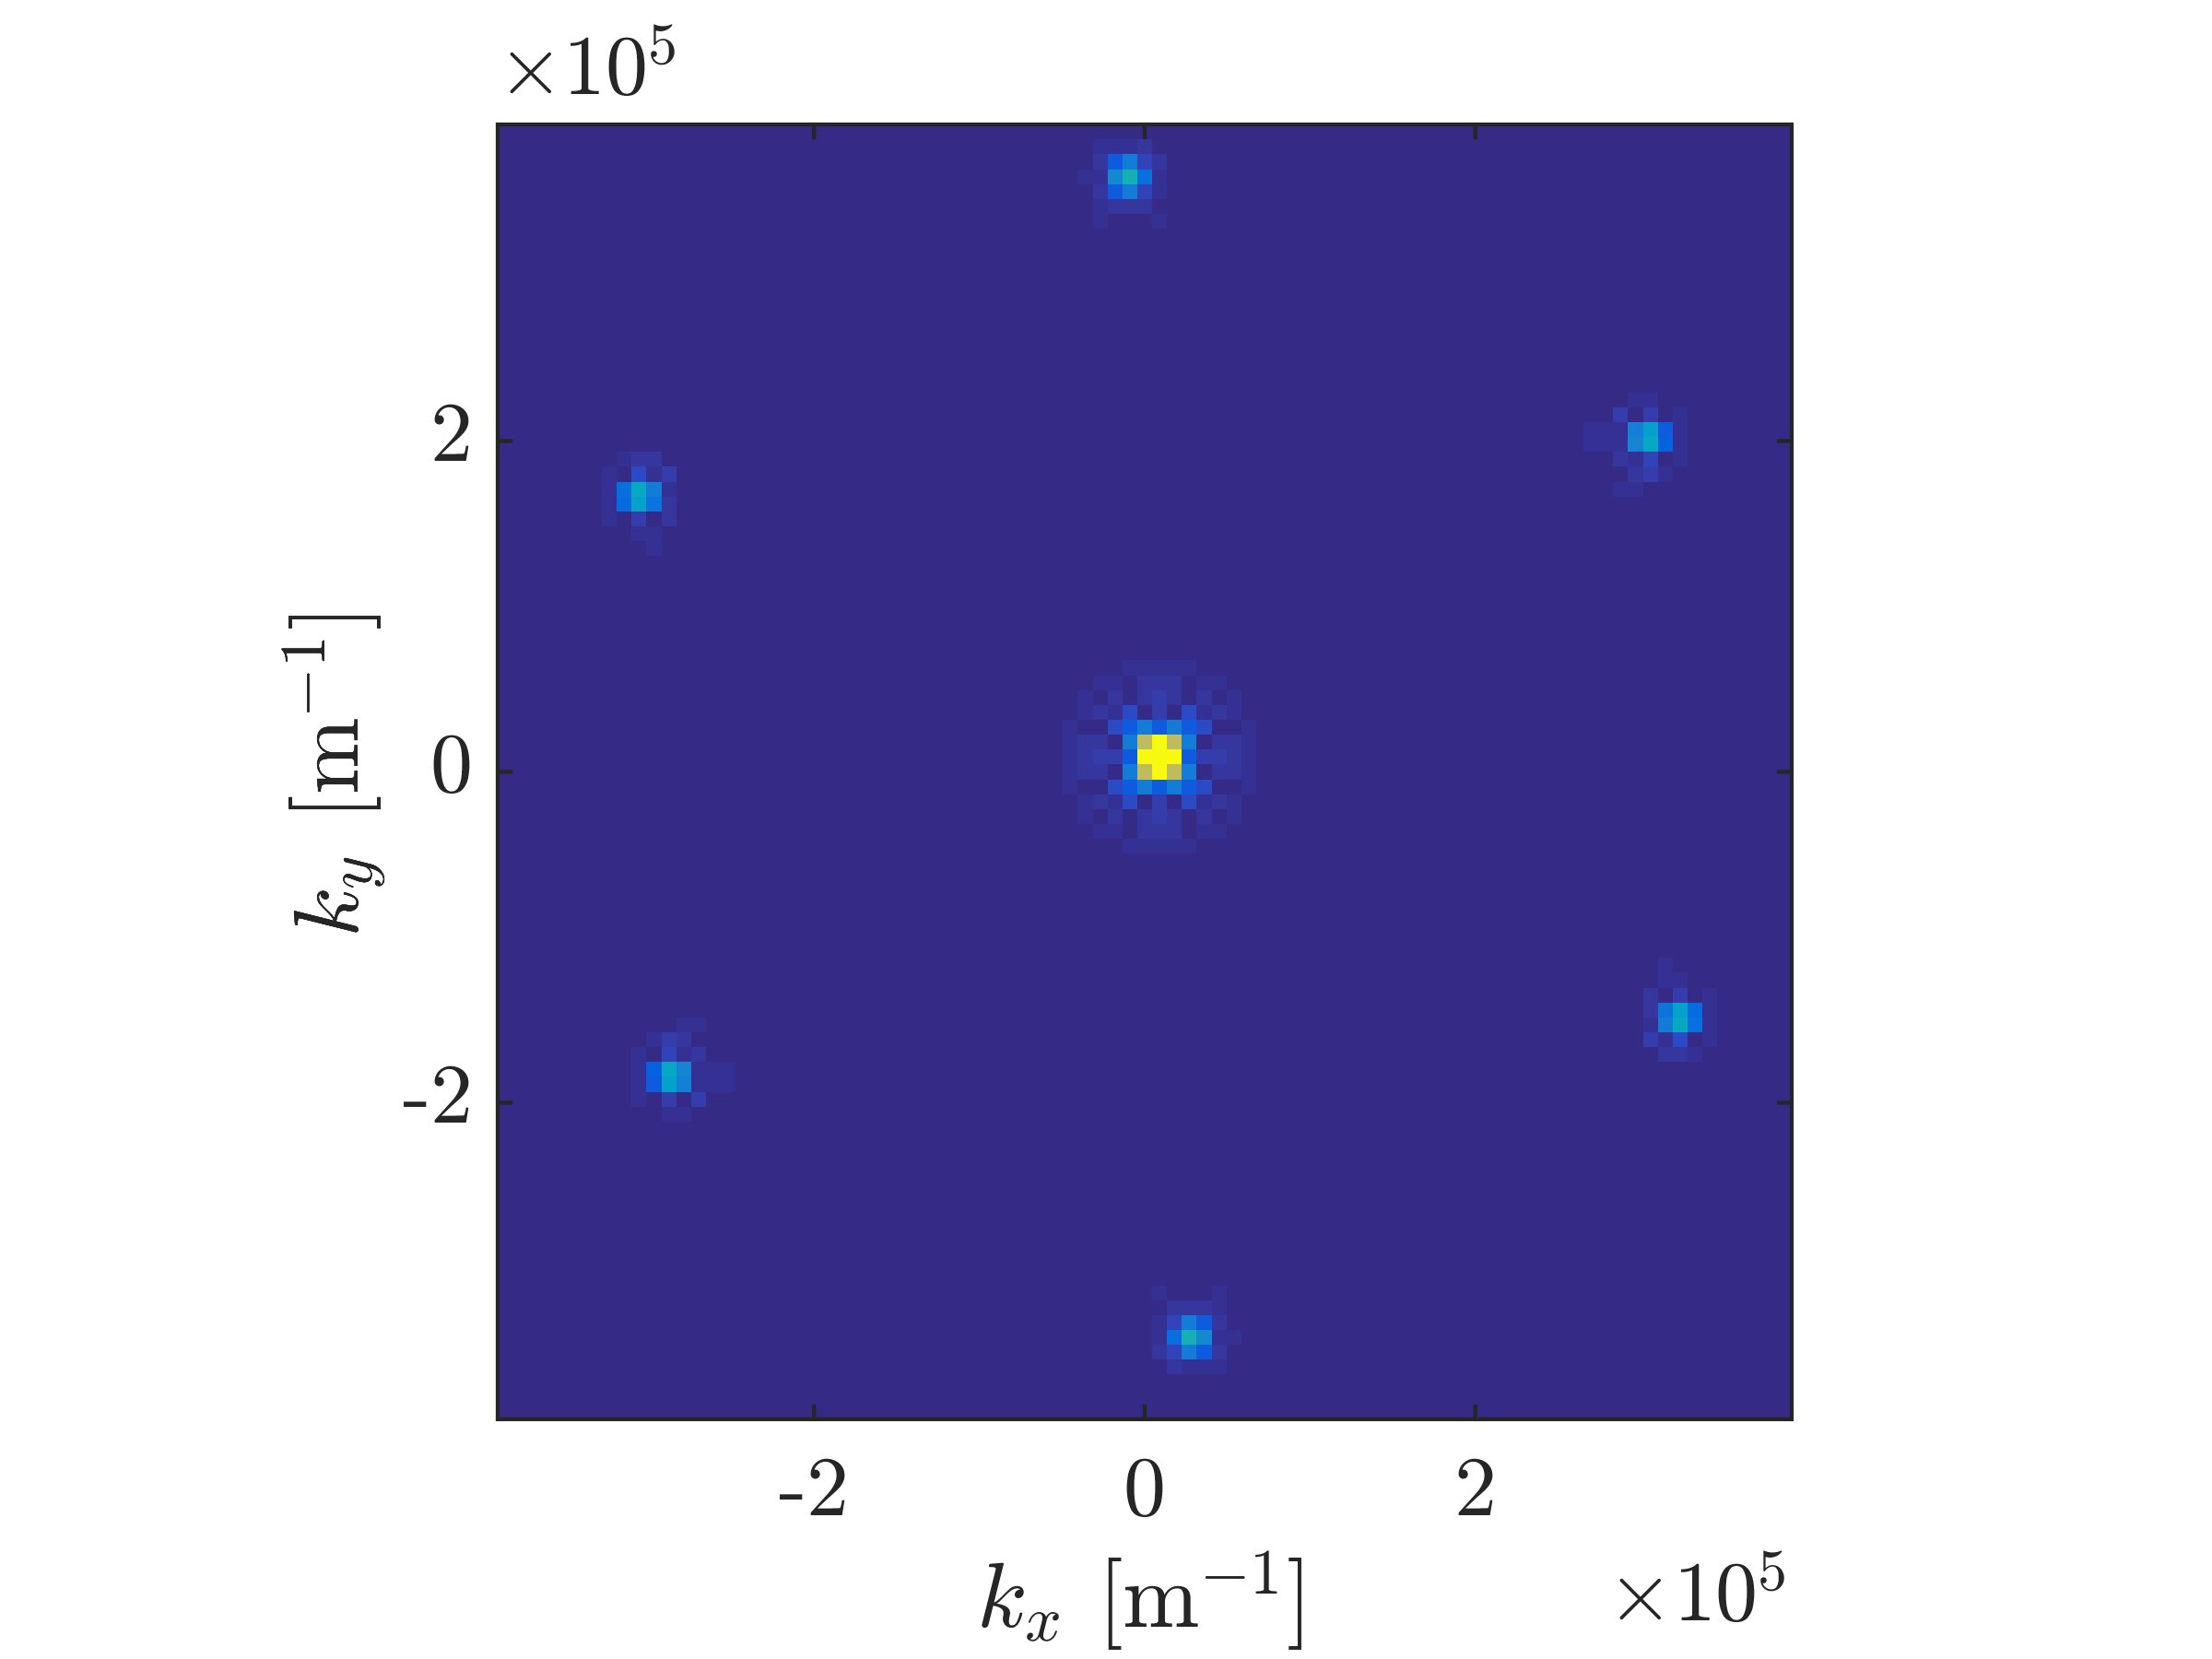
\includegraphics[width=0.48\textwidth]{imgs/FFT_density_linear_cell}
	\caption{Density structure factor within 4*pi/(sqrt(3)*d0).}
\end{figure}

%\begin{figure}[h!]
%	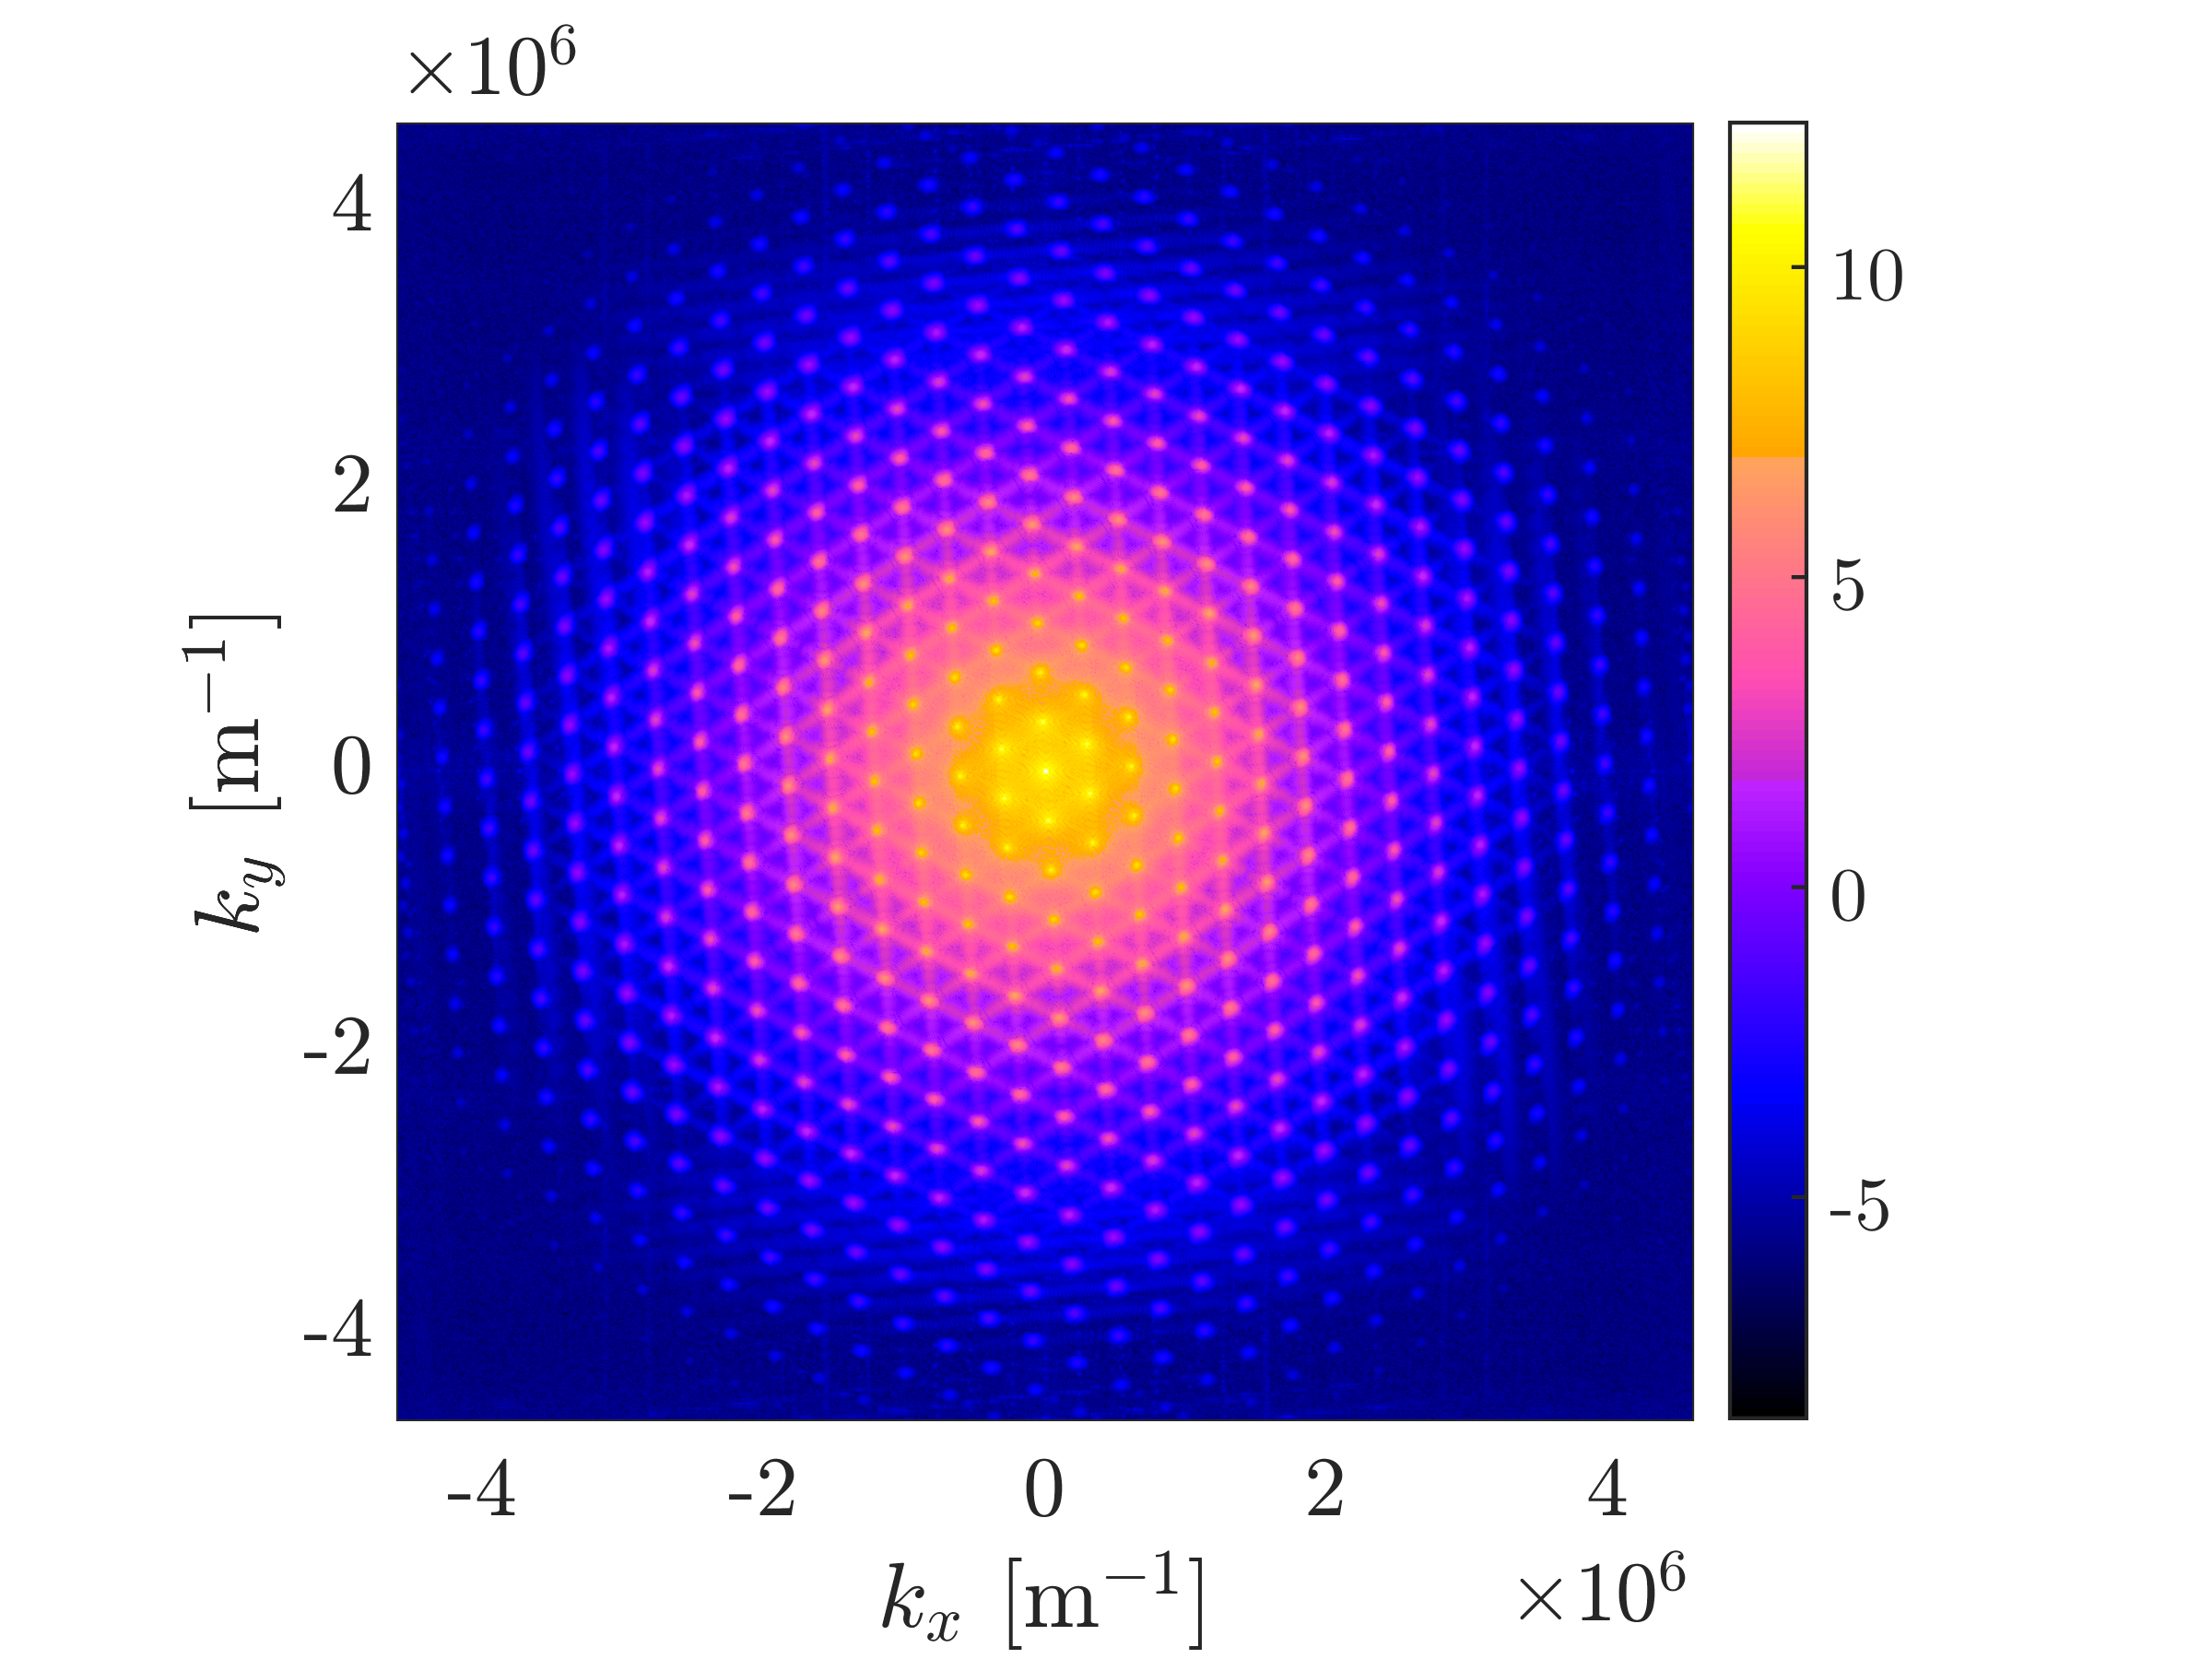
\includegraphics[width=0.48\textwidth]{imgs/FFT_density}
%	\caption{Density structure factor.}
%\end{figure}

\begin{figure}[tb]
	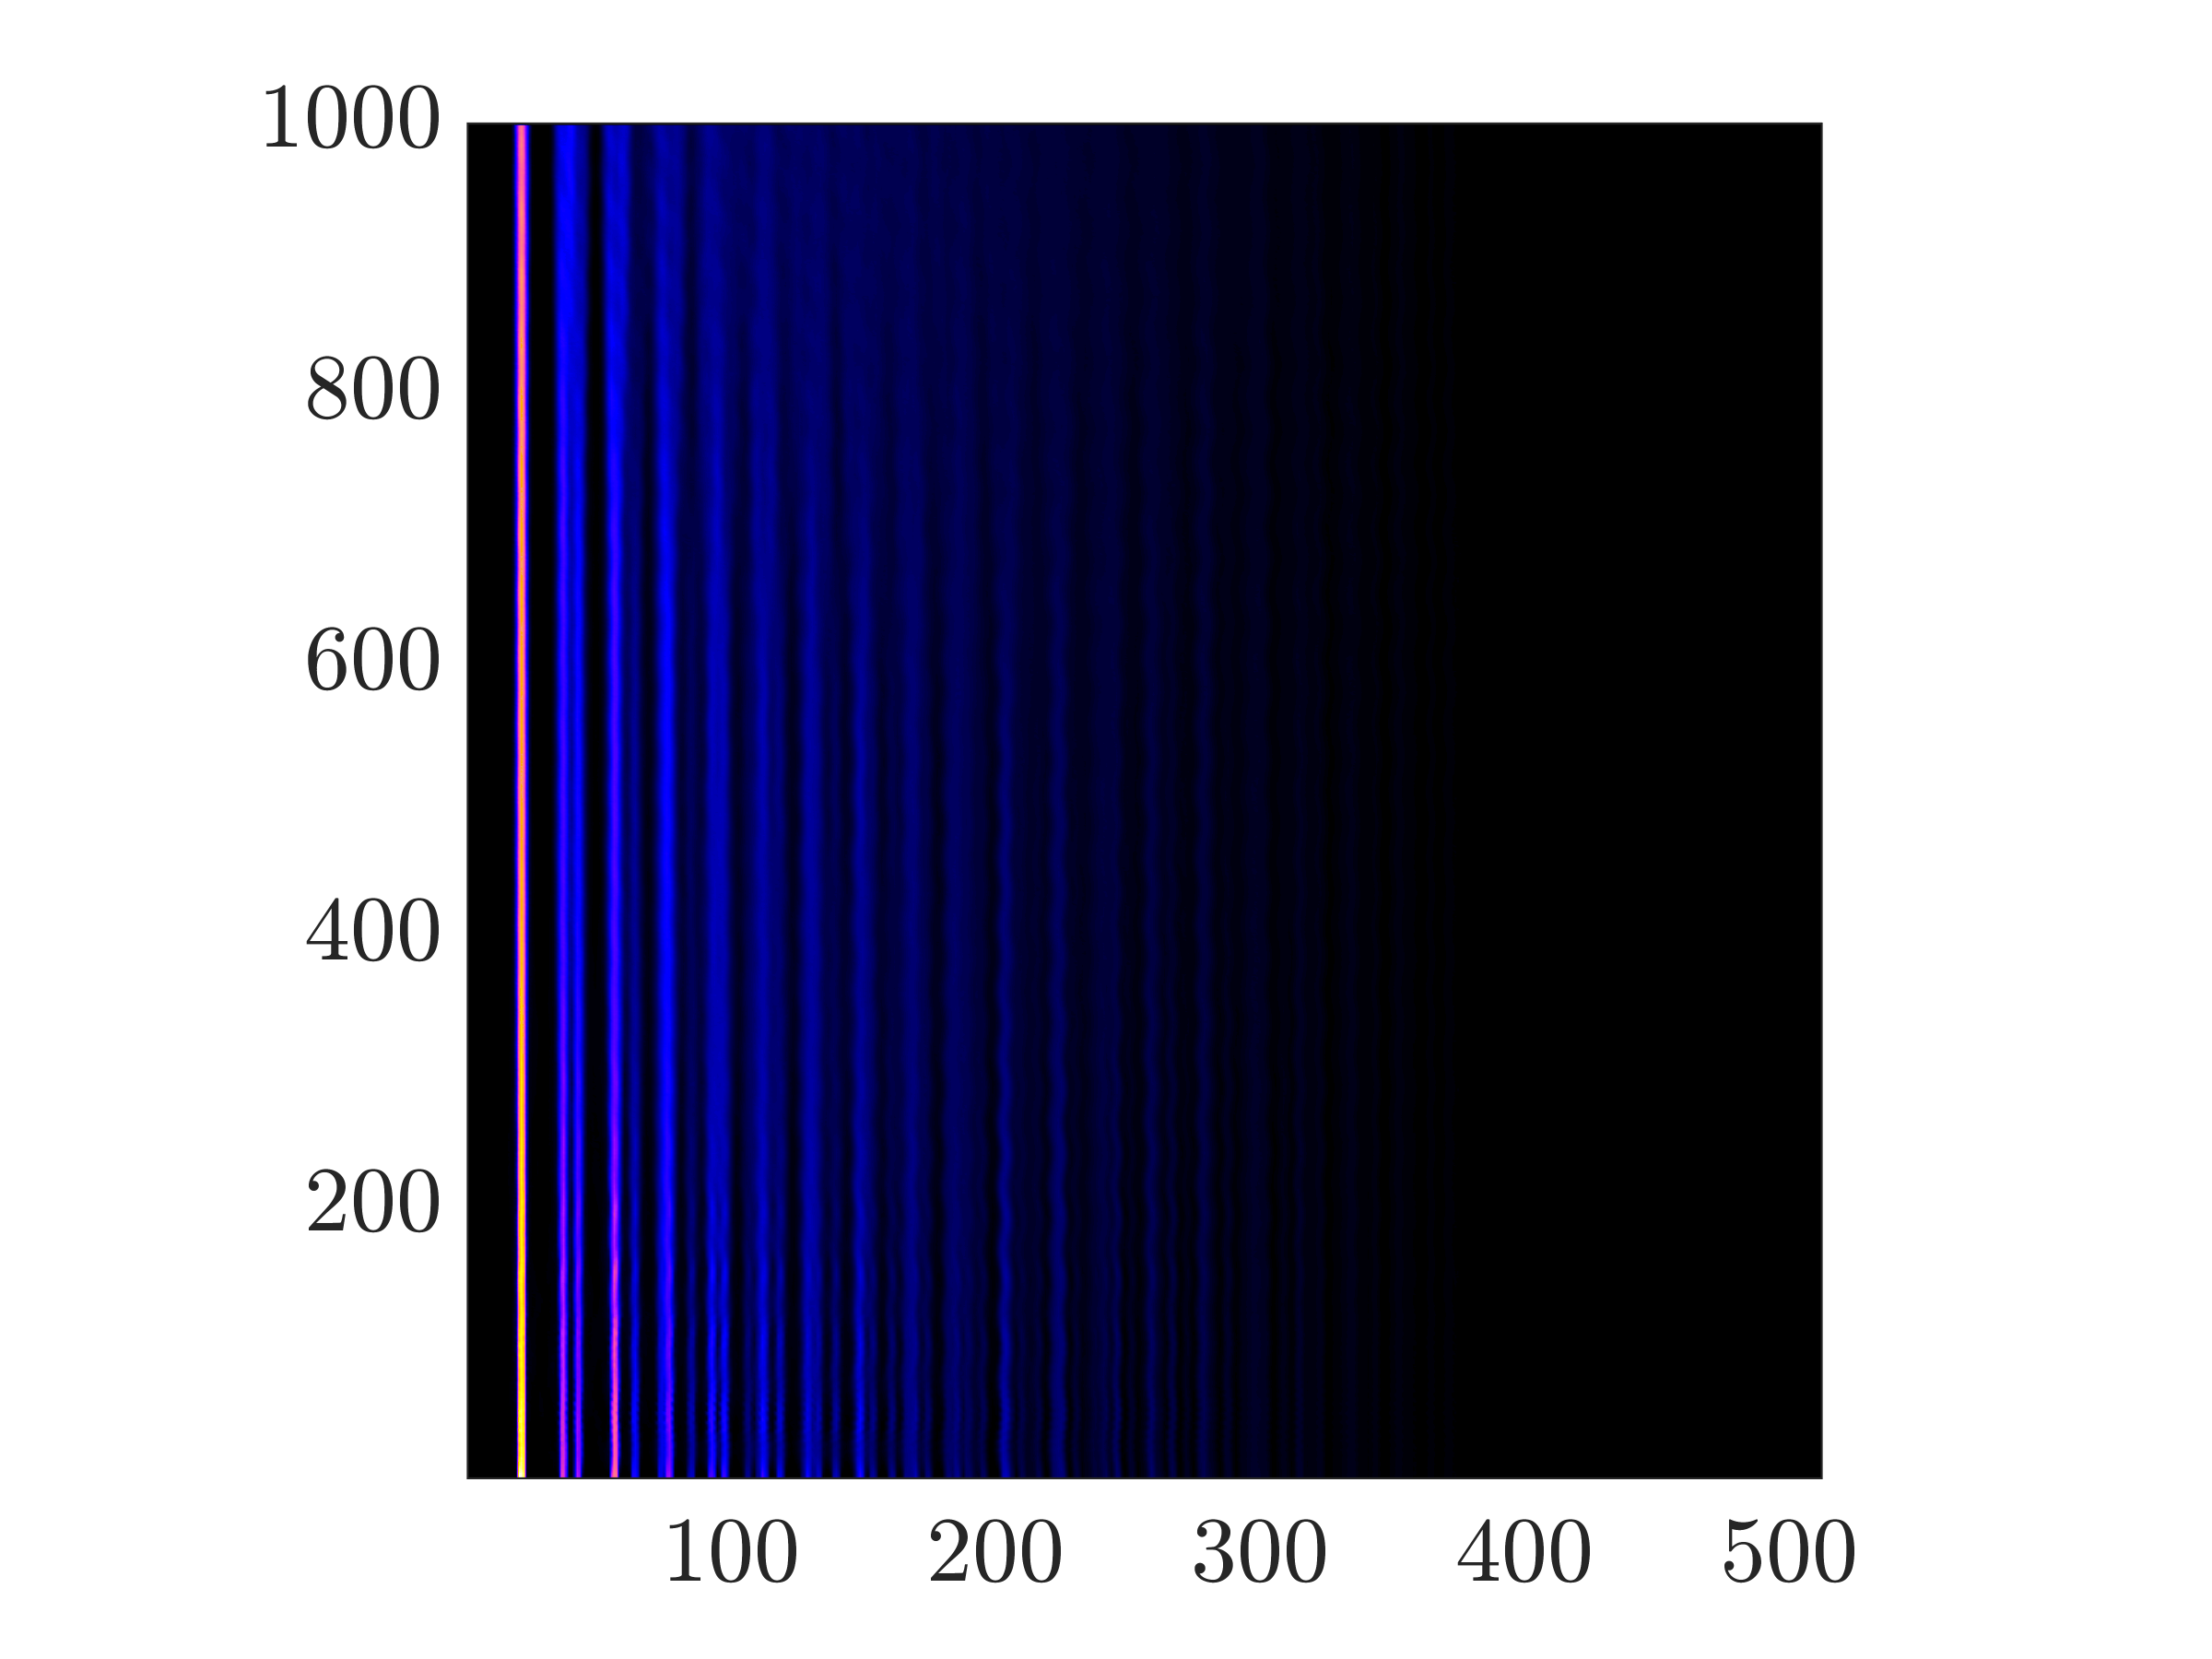
\includegraphics[width=0.48\textwidth]{imgs/RDF_time_gp}
	\caption{Radial distribution function over time after removing vortex from lattice centre. }
\end{figure}


\begin{figure}[tb]
	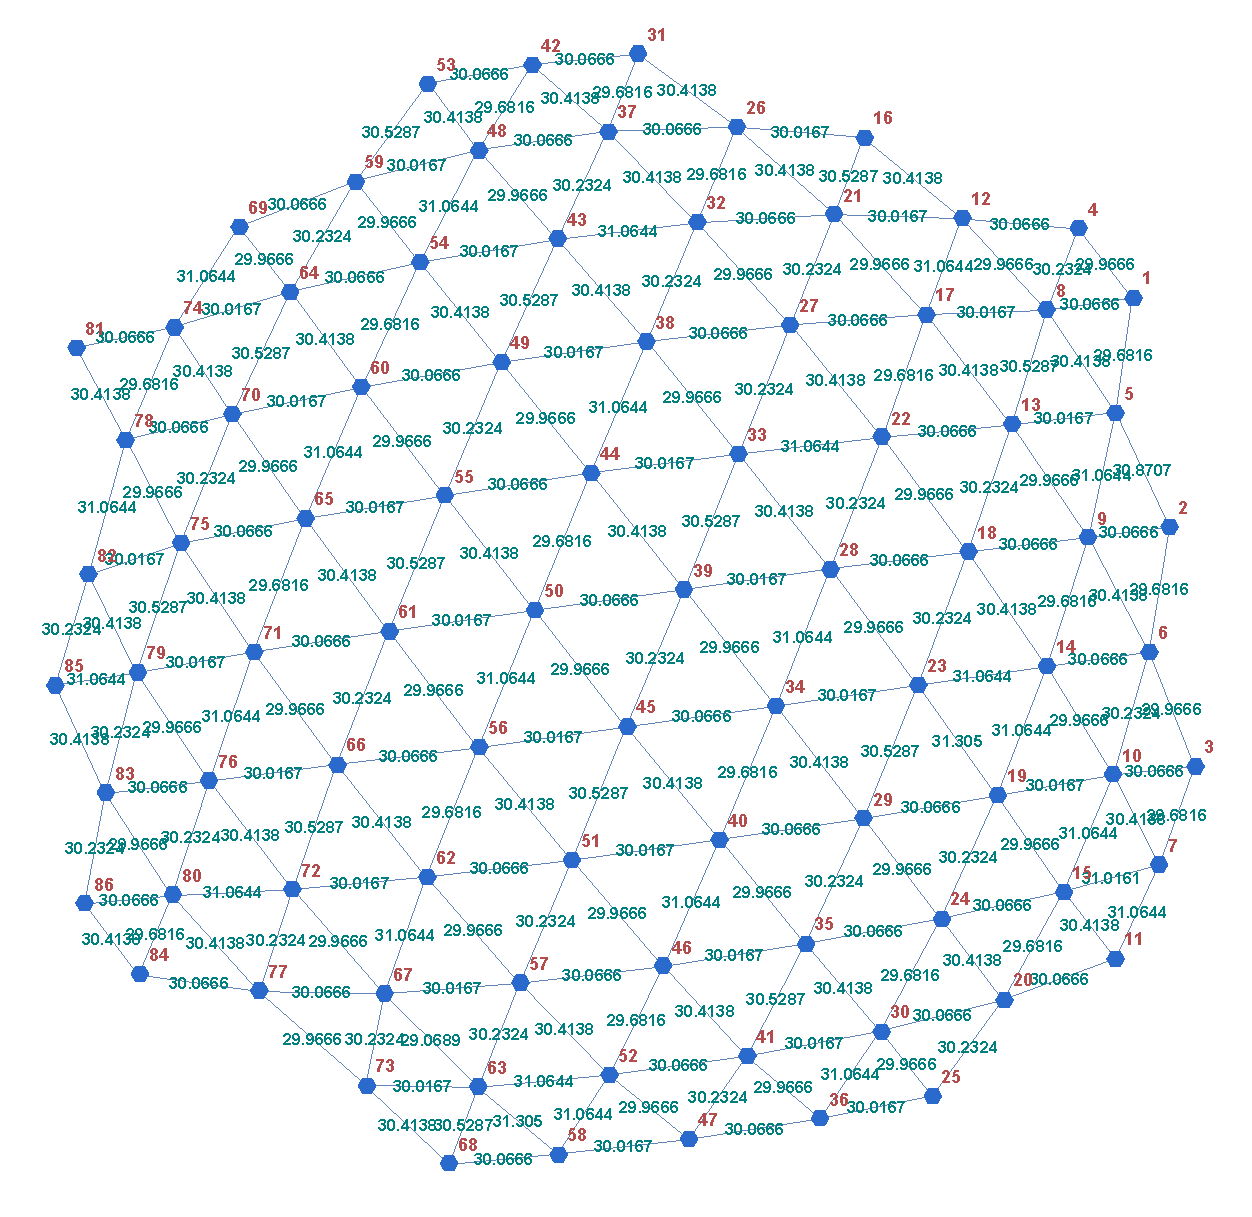
\includegraphics[width=0.48\textwidth]{imgs/graph86}
	\caption{Condensates vortices treated as nodes in a graph. Edges are drawn between nearest neighbours.}
\end{figure}
%\fi
%%%%%%%%%%%%%%%%%%%%%%%%%%%%%%%%%%%%%%%%%%%%%%%%%%%%%%%%%%%%%%%%%%%%%%%%%%%%%%%%%%%%%%%%%%%%%%%%%%%%%%%%%%%%%%%%%%%%%%%%%%%%%%%%%%%%%%%%%%%%%
\section{Conclusions}\label{sec:conc}
%%%%%%%%%%%%%%%%%%%%%%%%%%%%%%%%%%%%%%%%%%%%%%%%%%%%%%%%%%%%%%%%%%%%%%%%%%%%%%%%%%%%%%%%%%%%%%%%%%%%%%%%%%%%%%%%%%%%%%%%%%%%%%%%%%%%%%%%%%%%%

The removal of a vortex from the lattice creates a stable vacancy site, which in the corotating frame, travels with the lattice for some time
before decaying into paired 5 and 7 nearest neighbour disclinations. These disclination pairs can be viewed as as an edge dislocation in the
lattice. The resulting grain boundary breaks the 6-fold symmetry of the triangular lattice. The removal of the single vortex also removes the
velocity profile associated with the vortex at that location. The local velocity near the vacancy will be less than the solid-body behaviour
of the lattice. This causes the nearest neighbour vortices to rotate slower than the condensate, locally creating a strain/shear? on the
lattice. Local competition to fill the vacancy ensures its long-lived stability. The removal of the central vortex creates a local honeycomb
lattice structure, which according to [stat top of 2d lattice] will decay (following perturbation) via three possible processes.

Increasing the charge of a vortex by applying the same signed phase winding to a vortex core creates a stable doubly charged vortex for long
times (seconds). This, like the stable vacancy, seems to be stable at any range of positions (but decays faster at outskirts). The additional
velocity field shears the lattice, with the resulting correlations showing long-range power-law behaviour. This is usually indicative of a
power-law hexatic phase. Given the lack of true translational order in a harmonically trapped vortex lattice, it remains more instructive to
investigate the static structure factor of the system. The hexatic phase is expected to show spreading of the Fourier peaks into arcs. Here,
though we see such spreading, it is not entirely arc-like, and does not match entirely with the expectations of a hexatic phase.



%%%%%%%%%%%%%%%%%%%%%%%%%%%%%%%%%%%%%%%%%%%%%%%%%%%%%%%%%%%%%%%%%%%%%%%%%%%%%%%%%%
